\section{2. Přednáška}

% ============================================================
\subsection{Souvislost grafu a souvislé komponenty}
% ============================================================

Souvislost je jednou ze základních vlastností grafů. Díky ní víme, že z libovolného vrcholu $v$ se dostaneme do libovolného vrcholu $u$. \bigskip

\begin{definition}[Souvislý graf]
Neorientovaný graf $G$ je \textbf{souvislý}, jestliže v něm pro každé jeho dva vrcholy $u, v \in V(G)$ existuje $u$-$v$-cesta. Jinak je graf $G$ \textbf{nesouvislý}.
\end{definition} \bigskip

\noindent V případě, že je graf $G$ nesouvislý. Nás ale mohou zajímat jeho podgrafy, které již jsou souvislé. Ty se nazývají souvislé komponenty grafu $G$. \bigskip

\begin{definition}[Souvislá komponenta]
Indukovaný podgraf $H$ grafu $G$ je \textbf{souvislou komponentou}, pokud je souvislý a neexistuje žádný souvislý podgraf $F$ grafu $G$ takový, že $H \subseteq F$ a $H \neq F$.
\end{definition}

\noindent Souvislé komponenty jsou tedy největší možné podgrafy grafu $G$ takové, že jsou souvislé.

\begin{center}
    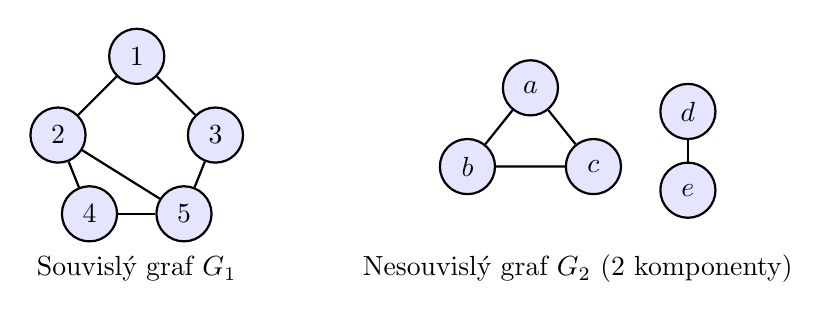
\begin{tikzpicture}[
  vnode/.style={circle, draw, minimum size=7mm, inner sep=0pt, fill=blue!10},
  thick
]
  % Souvislý graf G1 (vlevo)
  \begin{scope}[shift={(-3,0)}]
    \node[vnode] (1) at (0, 1.2) {1};
    \node[vnode] (2) at (-1, 0.2) {2};
    \node[vnode] (3) at (1, 0.2) {3};
    \node[vnode] (4) at (-0.6, -0.8) {4};
    \node[vnode] (5) at (0.6, -0.8) {5};
    \draw (1) -- (2); \draw (1) -- (3); \draw (2) -- (4); \draw (3) -- (5); \draw (4) -- (5); \draw (2) -- (5);
    \node at (0, -1.5) {Souvislý graf $G_1$};
  \end{scope}

  % Nesouvislý graf G2 (vpravo)
  \begin{scope}[shift={(3,0)}]
    % Komponenta A
    \node[vnode] (a) at (-1, 0.8) {$a$};
    \node[vnode] (b) at (-1.8, -0.2) {$b$};
    \node[vnode] (c) at (-0.2, -0.2) {$c$};
    \draw (a) -- (b) -- (c) -- (a);
    
    % Komponenta B
    \node[vnode] (d) at (1, 0.5) {$d$};
    \node[vnode] (e) at (1, -0.5) {$e$};
    \draw (d) -- (e);
    
    \node at (-0.4, -1.5) {Nesouvislý graf $G_2$ (2 komponenty)};
  \end{scope}
\end{tikzpicture}
\par\medskip
\textit{Obrázek 1.1: Ukázka souvislého grafu $G_1$ a nesouvislého grafu $G_2$ s dvěma komponentami indukovanými množinami $\{a,b,c\}$ a $\{d,e\}$.}
\end{center}

\begin{observation}
Graf je souvislý právě tehdy, když obsahuje jedinou souvislou komponentu.
\end{observation} 

\begin{observation}
Graf na $n$ vrcholech a 0 hranách má $n$ souvislých komponent.
\end{observation}

\bigskip

\noindent Souvislost lze také popsat pomocí relace ekvivalence na vrcholech grafu.

\begin{theorem}
Binární relace $\leftrightsquigarrow$ nad vrcholy grafu $G = (V, E)$ definovaná předpisem:
$$u \leftrightsquigarrow v \iff \text{existuje } u\text{-}v\text{-cesta v } G$$
je relací ekvivalence. Třídy ekvivalence této relace indukují souvislé komponenty grafu $G$.
\end{theorem} \bigskip

\noindent Předtím, než se podíváte na důkaz přoč je tato relace ekvivalencí, zkuste si to jako cvičení dokázat sami, u prvních dvou vlastností se jedná se o velmi přímočarý důkaz a velmi dobré cvičení na ověření si, zda jste tuto definici správně pochopili. U třetí vlastnosti si pak musíte uvědomit, že složením dvou cest nemusí vzniknout cesta, ale sled (ten pak lze zkrátit na cestu, na tento důkaz narazíme v druhé půlce semestru).

\begin{proof}
    Stačí nám ověřit reflexivitu, symetrii a transitivitu (viz. DML), tím dokážeme ekvivalenci. \\
    
    \noindent Mějme graf $G$ a nějaké jeho 3 vrcholy $u, v, w \in G$.

    \begin{enumerate}
        \item Reflexivita - Z vrcholu $v$ určitě existuje cesta do vrcholu $v$. Je to    přesně cesta délky 0.
        \item Symetrie - Pokud existuje $u$-$v$-cesta, tak využitím stejný hran a          vnitřních vrcholů. Pouze nyní směrem z vrcholu $u$ do vrcholu $v$. Získáme hledanou $v$-$u$-cestu.
        \item Transitivita - Pokud existuje $u$-$v$-cesta a $v$-$w$-cesta, tak poté spojením těchto dvou cest nám vznikne sled z $u$ do $w$. Ten lze ale zkrátit na cestu (to je netriviální, důkaz v 10. přednášce).
    \end{enumerate}
\end{proof}

% ==================================================================
\subsection{Rozklad grafu na souvislé komponenty (BFS\_Graf)}
% ==================================================================

Pokud graf tedy není souvislý, nemůžeme jednodušše pustit algoritmus BFS na libovolném vrcholu a očekávat, že nalezne všechny vrcholy, jak to tedy zařídit? Zařídí to tato mírně modifikovaná verze algoritmu.

\noindent Algoritmus \texttt{BFS\_Graf} prochází celý graf $G$ a postupně spouští algoritmus BFS pro každý dosud nenalezený vrchol $s \in V(G)$. Tímto způsobem postupně projde všechny souvislé komponenty grafu a spočítá vzdálenosti $D$ i strom nejkratších cest $P$ pro každou komponentu zvlášť. Nemůže tak zůstat vrchol do, kterého by se algoritmus nedostal, jelikož bude provolán vnější smyčkou a sám najde všechny ze svojí komponenty. \bigskip

\begin{remark}
    Toto není jediný způsob prohledání grafu, algoritmus BFS lze v tomto případě například zaměnit za DFS.
\end{remark} \bigskip

\noindent \textbf{Vstup}: Neorientovaný graf $G = (V, E)$. \newline
\noindent \textbf{Výstup}: 
\begin{itemize}[itemsep=-0.2em, topsep=0.1em]
    \item Pole vzdáleností $D$ pro všechny vrcholy $v \in V(G)$ od startovních vrcholů jejich příslušných souvislých komponent.
    \item Pole předchůdců $P$ určující stromy nejkratších cest v jednotlivých komponentách.
\end{itemize}

\bigskip
\funkce{BFS\_Graf}{graf $G$}
\begin{pseudocode}
\item Pro každý vrchol $u \in V(G)$:
\item \tab $\text{stav}[u] := \text{nenalezený}$
\item \tab $D[u] := \text{undef}$
\item \tab $P[u] := \text{undef}$
\item Pro každý vrchol $s \in V(G)$:
\item \tab Pokud $\text{stav}[s] = \text{nenalezený}$:
\item \tab \tab Zavolej \textcolor{blue}{BFS}($G, s$)
\item Vrať $(D, P)$
\end{pseudocode} \bigskip

\begin{proof}[Důkaz Korektnosti algoritmu BFS\_Graf]
    Dokážeme přímo
    \begin{enumerate}
        \item U algoritmus BFS jsme již dokázali, že správně vyplní pole předchůdců, pole vzdáleností a nevynechá žádný vrchol.
        
        \item Algoritmus BFS\_Graf nejprve nastaví všechny vrcholy na stav \textit{nenalezený}. Poté postupně prochází všechny vrcholy $s \in V(G)$. Pokud je vrchol $s$ stále nenalezený, zavolá na něm algoritmus BFS.

        \item Uvažujme libovolnou komponentu souvislosti $C$ grafu $G$. Pokud ještě žádný vrchol z $C$ nebyl nalezen, algoritmus při průchodu vrcholů narazí na některý vrchol $s \in C$ ve stavu \textit{nenalezený} a zavolá BFS$(G,s)$. Protože všechny vrcholy v $C$ jsou z $s$ dosažitelné, algoritmus BFS nalezne všechny vrcholy komponenty $C$.
        
        \item Po dokončení tohoto volání jsou všechny vrcholy komponenty $C$ označeny jako uzavřené. Když tedy algoritmus později narazí na další vrchol z této komponenty, podmínka $\text{stav}[s] = \text{nenalezený}$ již nebude splněna a další volání BFS nebude provedeno.
        
        \item Každá komponenta souvislosti je tedy zpracována právě jedním voláním algoritmu BFS a žádná komponenta není vynechána. Jelikož je BFS korektní, jsou pro všechny vrcholy správně určeny hodnoty $D$ a $P$.

        \item Algoritmus BFS\_Graf je proto korektní.
    \end{enumerate}
\end{proof}

\noindent Teď tedy víme, jak prohledat celý graf i pokud předem nevíme, zda je souvislý. Můžete se ale ptát, jak ověřit souvislost grafu? Jak najít jeho souvislé komponenty? Pokud dostanu zadaný vrchol jak najít jeho komponentu souvislosti? Na tyto otázky nyní odpovíme malým "vylepšením" algoritmu, který jsme si právě ukázali. \\

\noindent Dostaneme-li vrchol $s$ jak najít jeho souvislou komponentu? K tomuto nám stačí algoritmus který jsme si právě ukázali, stačí jen přidat jedno pole identifikátorů které pro každý vrchol držet identifikátor komponenty souvislosti ve které se vrchol nachází, to algoritmus vyplní vrcholem ve kterém začalo prohledávání současné komponenty.

\newpage

% ============================================================
\subsection{Výpočetní model RAM}
% ============================================================

Z PAx jistě znáte časovou a paměťovou složitost programu. Abychom ale mohli analyzovat složitosti algoritmu, musíme si zadefinovat nějaký model počítače. Počítače se často hodně liší, různé istrukce trvají jinak dlouho, atd. Proto si zavedeme teoretický model počítače, který modeluje to, co všichni přibližně od běžného počítače očekáváme.

\begin{definition}[Model RAM]
Výpočetní model \textbf{RAM} se skládá ze dvou hlavních částí:
\begin{itemize}
    \item \textbf{Paměť}: Je tvořena adresovatelným polem celočíselných paměťových buněk. Adresy jsou celá čísla.
    \item \textbf{Program}: Je konečná posloupnost sekvenčně prováděných instrukcí. Instrukce dělíme na:
    \begin{enumerate}
        \item \textbf{Aritmeticko-logické:} (sčítání, násobení, porovnávání, ...): Obvykle mají dva vstupní argumenty a jeden výstupní. Vstupem může být přímá konstanta, přímo adresovaná buňka, nebo nepřímo adresovaná buňka (adresa je uložena v jiné přímo adresované buňce).
        \item \textbf{Řídicí}: Zahrnují nepodmíněné skoky, podmíněné skoky a instrukci pro zastavení programu (halt).
    \end{enumerate}
\end{itemize}
\end{definition} \medskip

\noindent Na začátku výpočtu jsou vstupní data uložena v určených paměťových buňkách a procesor v každém kroku provede právě jednu instrukci. Po zastavení se obsah určených buněk interpretuje jako výstup. 

\medskip

\begin{remark}
    Pro představu může sloužit např. Assembler z předmětu SAP nebo APS. ADD je příkladem aritmeticko-logické instrukce a JMP příkladem řídící instrukce. Na vstup dostanou buďto konstantu, registr, nebo hodnotu z paměti.
\end{remark}

\bigskip

\noindent Nyní se konečně dostáváme k tomu co je časová a paměťová složitost. Je to ten nejhorší případ, ze všech vstupů až do velikosti $n$ včetně.

\medskip

\begin{definition}[Složitost programu v modelu RAM]
Složitost algoritmu v nejhorším případě pro vstup velikosti $n$ definujeme následovně:
\begin{itemize}
    \item \textbf{Velikost vstupu $n$} je počet paměťových buněk, které vstup zabírá.
    \item \textbf{Časová složitost} je maximum z počtu vykonaných instrukcí přes všechny povolené vstupy velikosti nejvýše $n$.
    \item \textbf{Paměťová (prostorová) složitost} je maximum z počtu použitých paměťových buněk přes všechny povolené vstupy velikosti nejvýše $n$.
\end{itemize}
\end{definition}


\noindent Co nás bude u algoritmů zajímat je, jak budou složitosti programu škálovat s velikostí vstupu, tedy nebudeme počítat přesný počet instrukcí, ale spíše zda algoritmus vykoná za jeho běh $\mathcal{O}(n)$ instrukcí nebo třeba $\mathcal{O}(n^2) \text{ či dokonce } \mathcal{O}(2^n)$.

% ============================================================
\subsection{Reprezentace grafů v paměti počítače}
% ============================================================

Samotný graf můžeme v modelu RAM reprezentovat různými způsoby. Některé způsoby jsou lepší na rychlejší vyhledávání, jiné třeba víc spoří pamětí. Při programování zvolte způsob dle vašich požadavků. Zde si představíme dva možné a to matici sousednosti a seznam sousedů. \bigskip

\subsubsection{Matice sousednosti}
\begin{definition}[Matice sousednosti]
Nechť $G = (V, E)$ je neorientovaný graf s množinou vrcholů $V = \{v_1, v_2, \dots, v_n\}$. \textbf{Matice sousednosti} grafu $G$ je čtvercová matice $A_G = (a_{i,j})_{i,j=1}^n$ typu $n \times n$ definovaná předpisem:
$$a_{i,j} = \begin{cases} 1 & \text{pokud } \{v_i, v_j\} \in E, \\ 0 & \text{jinak.} \end{cases}$$
\end{definition} \bigskip

\begin{remark}
Pro neorientovaný graf je matice $A_G$ vždy symetrická podle hlavní diagonály. Diagonální prvky $a_{i,i}$ jsou nulové (neorientovaný graf nemá smyčky). Paměťová složitost této reprezentace je vždy \textbf{$\bigO{n^2}$}, což je nevýhodné pro řídké grafy ($m \ll n^2$). Výhodou je zarovnaný přístup do paměti a díky tomu i dobrá cache.
\end{remark} \bigskip

\subsubsection{Seznam sousedů}
\begin{definition}[Seznam sousedů]
V reprezentaci \textbf{seznamem sousedů} uchováváme pro každý vrchol $v \in V(G)$ jednosměrně či obousměrně zřetězený seznam všech jeho sousedů (tedy vrcholů $w$, pro které $\{v, w\} \in E$).
\end{definition} \bigskip

\begin{remark}
Paměťová složitost se skládá z pole o velikosti $|V| = n$ pro začátky seznamů a z celkem $2|E| = 2m$ prvků v seznamech (každá neorientovaná hrana je uložena dvakrát -- u obou svých koncových vrcholů). Celková paměťová složitost je tedy \textbf{$\bigO{n + m}$}, což je optimální a velmi efektivní pro řídké grafy. V progtestech jsem volil tento způsob a prošel mi naprosto v pohodě:D
\end{remark} \bigskip

\subsubsection{Reprezentace orientovaného grafu}
U orientovaných grafů reprezentujeme hrany jako uspořádané dvojice:
\begin{itemize}
    \item \textbf{Matice sousednosti} obsahuje $a_{i,j} = 1$ právě tehdy, když v grafu existuje orientovaná hrana $(v_i, v_j) \in E$. Tato matice obecně \textbf{není symetrická}.
    \item \textbf{Seznam sousedů} nahrazujeme \textbf{seznamem následníků}: pro každý vrchol $v$ ukládáme pouze seznam vrcholů $w$ takových, že do nich vede orientovaná hrana $(v, w) \in E$. Celkový počet prvků v seznamech je právě $|E| = m$.
\end{itemize} \bigskip

\begin{center}
    
\usetikzlibrary{shapes.geometric, positioning, arrows.meta, matrix}

\begin{figure}[H]
\centering
\large $G = (\{0, 1, 2, 3\}, \{(0, 1), (0, 2), (2, 1), (3, 2)\})$
\vspace{6mm}

\begin{tikzpicture}[
  vnode/.style={circle, draw, minimum size=7mm, inner sep=0pt},
  boxnode/.style={rectangle, draw, minimum size=6mm, inner sep=0pt, anchor=center},
  thick,
  >=stealth
]
  % (a) Orientovaný graf G
  \begin{scope}[shift={(0,0)}]
    \node[vnode] (0) at (0, 1.5) {0};
    \node[vnode] (3) at (1.5, 1.5) {3};
    \node[vnode] (1) at (0, 0) {1};
    \node[vnode] (2) at (1.5, 0) {2};

    \draw[->] (0) -- (1);
    \draw[->] (0) -- (2);
    \draw[->] (3) -- (2);
    \draw[->] (2) -- (1);

    \node at (0.75, -0.9) {Orientovaný graf $G$};
  \end{scope}

  % (b) Matice sousednosti A_G
  \begin{scope}[shift={(5.0,0)}]
    \node (m) at (0.9,0.75) {
      \begin{tabular}{|c|c|c|c|}\hline
      0 & 1 & 1 & 0 \\
      0 & 0 & 0 & 0 \\
      0 & 1 & 0 & 0 \\
      0 & 0 & 1 & 0 \\\hline
      \end{tabular}
    };

    % Popisky řádků a sloupců (removed due to matrix replacement)

    \node at (0.9, -0.9) {Matice sousednosti $A_G$};
  \end{scope}

  % (c) Seznam následníků
  \begin{scope}[shift={(10.2,0)}]
    % Levý sloupec vrcholů (0, 2, 3)
    \node[boxnode] (h0) at (0, 1.35) {0};
    \node[boxnode, below=-\pgflinewidth of h0] (h2) {2};
    \node[boxnode, below=-\pgflinewidth of h2] (h3) {3};

    % Řádek 0:
    \node[boxnode, right=6mm of h0] (l01) {1};
    \node[boxnode, right=-\pgflinewidth of l01] (l02) {2};
    \draw[->] (h0) -- (l01);

    % Řádek 2:
    \node[boxnode, right=6mm of h2] (l21) {1};
    \draw[->] (h2) -- (l21);

    % Řádek 3:
    \node[boxnode, right=6mm of h3] (l32) {2};
    \draw[->] (h3) -- (l32);

    \node at (0.8, -0.9) {Seznam následníků};
  \end{scope}

\end{tikzpicture}
\caption{Orientovaný graf $G$ a jeho reprezentace maticí sousednosti a seznamem následníků.}
\label{fig:orientovany-graf-reprezentace}
\end{figure}

\end{center}

% ============================================================
\subsection{Časová složitost algoritmu BFS}
% ============================================================

Díky zavedení modelu RAM nyní můžeme konečně dokázat časovou složitost algoritmu BFS
Na základě definovaného modelu RAM a reprezentace grafu můžeme exaktně dokázat časovou složitost algoritmu BFS. 

\medskip

\begin{theorem}[O časové složitosti algoritmu BFS]
Algoritmus $BFS(G, s)$ má při reprezentaci grafu $G$ seznamem sousedů časovou složitost $\bigO{|V| + |E|}$.
\end{theorem} 

\begin{proof}
Časovou složitost můžeme rozdělit na analýzu jednotlivých fází algoritmu:
\begin{enumerate}
    \item \textbf{Inicializace} (řádky 1--3 a 5--6 v neorientované verzi):
    \begin{itemize}
        \item Procházíme všechny vrcholy a na každém provedeme konstantě mnoho práce. Nastavujeme jejich stav na \textit{nenalezený}, vzdálenost na \textit{undef} a předchůdce na \textit{undef}. Celkem to stihneme za $\bigO{|V|}$.
    \end{itemize}
    \item \textbf{Práce s frontou $Q$} (hlavní cyklus na řádcích 7--15):
    \begin{itemize}
        \item Každý vrchol $v \in V(G)$ je do fronty $Q$ přidán nejvýše jednou, protože se jeho stav bezprostředně před vložením změní na \textit{otevřený}. Vrchol v tomto stavu již nemůže splnit podmínku na řádku 10 a do fronty se podruhé nedostane.
        \item V každé iteraci hlavního cyklu je právě jeden vrchol z fronty odebrán. Hlavní cyklus se tedy provede nejvýše $|V|$-krát. Každá operace s frontou zabere konstantní množství času. Tedy celkem $\bigO{|V|}$.
    \end{itemize}
    \item \textbf{Prohledávání sousedů} (vnitřní cyklus na řádcích 9--14):
    \begin{itemize}
        \item Když je vrchol $v$ vyjmut z fronty, projdeme celý jeho seznam sousedů. Což je nejhůře až $\bigO{|E|}$.
        \item V neorientovaném grafu se na každou hranu podíváme nejvýše dvakrát (jednou z každého jejího koncového vrcholu). Celkový počet zpracování hran je tedy nejvýše $2|E|$, což je $\bigO{|E|}$.
    \end{itemize}
\end{enumerate}
Celkem tedy dostáváme $\bigO{|V| + |E|}$.
\end{proof} \bigskip

\noindent Je důležité opravdu psát $\bigO{|V| + |E|}$ a ne jen $\bigO{|V|} \text{ nebo } \bigO{|E|}$, protože nevíme, zda je v grafu více vrcholů nebo hran. Také je dobré si uvědomit, že počet hran v grafu může být až kvadrát počtu vrcholů. 

\medskip

\begin{theorem}[O časové složitosti algoritmu BFS\_Graf]
Algoritmus $BFS\_graf(G)$, má při reprezentaci grafu seznamem sousedů celkovou časovou složitost $\bigO{|V| + |E|}$.
\end{theorem}

\medskip

\begin{proof}
Algoritmus vnějším cyklem projde všechny vrcholy $v \in V(G)$ postupně. Zvolme si libovolnou komponentu souvislosti $C$ grafu $G$. V jednom z vrcholů zacněme BFS a projdeme jí za $\bigO{|V(C)| + |E(C)|}$. Jelikož komponenty nemají žádnou společnou část. Tedy průchodem nic neopakujeme. Tak projdeme celý graf za sumu přes všechny komponenty. Což je právě celý graf. Tedy $\bigO{|V| + |E|}$.
\end{proof}

\newpage

% ============================================================
\subsection{Slabá a silná souvislost orientovaných grafů}
% ============================================================

Pro orientované grafy je potřeba pojem souvislosti trochu rozšířit. Rozlišujeme dva druhy. Slabou a silnou souvislost. U Slabé souvislosti se ke hranám chováme, jako by byly neorientované. U Silné souvislosti naopak požadujeme, aby existovala orientovaná cesta mezi libovolnými dvěma vrcholy. Prvně si zavedeme pomocnou definici a to symetrizaci grafu neboli to již zmiňované ignorování orientace hran. \medskip

\begin{definition}[Symetrizace orientovaného grafu]
Nechť $G = (V, E)$ je orientovaný graf. \textbf{Symetrizace} grafu $G$ je neorientovaný graf $sym(G) = (V, E')$, kde pro každé dva vrcholy $u, v \in V$ platí:
$$\{u, v\} \in E' \iff (u, v) \in E \lor (v, u) \in E$$
\end{definition} 

\medskip

\begin{definition}[Slabá souvislost]
Orientovaný graf $G$ je \textbf{slabě souvislý}, pokud je souvislá jeho symetrizace $sym(G)$.
\end{definition} 

\medskip

\begin{definition}[Silná souvislost]
Orientovaný graf $G = (V, E)$ je \textbf{silně souvislý}, pokud pro každé dva vrcholy $u, v \in V$ existuje v $G$ orientovaná cesta z $u$ do $v$ a zároveň orientovaná cesta z $v$ do $u$.
\end{definition} 

\medskip

\begin{center}
    \begin{figure}[H]
\centering
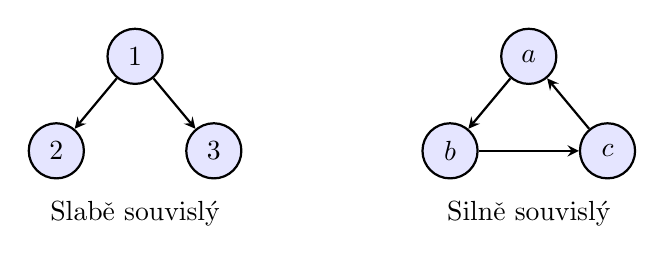
\begin{tikzpicture}[
  vnode/.style={circle, draw, minimum size=7mm, inner sep=0pt, fill=blue!10},
  thick,
  >=stealth
]
  % Slabě souvislý (vlevo)
  \begin{scope}[shift={(-2.5,0)}]
    \node[vnode] (1) at (0, 0.8) {1};
    \node[vnode] (2) at (-1, -0.4) {2};
    \node[vnode] (3) at (1, -0.4) {3};
    \draw[->] (1) -- (2);
    \draw[->] (1) -- (3);
    \node at (0, -1.2) {Slabě souvislý};
  \end{scope}

  % Silně souvislý (vpravo)
  \begin{scope}[shift={(2.5,0)}]
    \node[vnode] (a) at (0, 0.8) {$a$};
    \node[vnode] (b) at (-1, -0.4) {$b$};
    \node[vnode] (c) at (1, -0.4) {$c$};
    \draw[->] (a) -- (b);
    \draw[->] (b) -- (c);
    \draw[->] (c) -- (a);
    \node at (0, -1.2) {Silně souvislý};
  \end{scope}
\end{tikzpicture}
\caption{Ukázka slabě souvislého grafu (z vrcholu 2 se nelze dostat nikam, ale po ignorování šipek je souvislý) a silně souvislého grafu (obsahuje orientovaný cyklus).}
\end{figure}
\end{center}

% ============================================================
\subsection{Izomorfismus a automorfismus grafů}
% ============================================================

Často se může stát, kdy se bavíme o dvou grafech, které jsou strukturou identické, ale jsou například jinak nakreslené nebo pokud mají jinak označené vrcholy. Abychom vyjádřili do jisté míry rovnost těchto grafů, zavádíme následující pojmy. \bigskip

\begin{definition}[Izomorfismus grafů]
Nechť $G$ a $H$ jsou dva grafy. Zobrazení $f : V(G) \to V(H)$ nazveme \textbf{izomorfismem grafů} $G$ a $H$, pokud platí:
\begin{enumerate}
    \item $f$ je bijekce
    \item pro každou dvojici vrcholů $u, v \in V(G)$ platí:
    $$\{u, v\} \in E(G) \iff \{f(u), f(v)\} \in E(H)$$
\end{enumerate}
Pokud takové zobrazení existuje, říkáme, že grafy $G$ a $H$ jsou \textbf{izomorfní} and značíme $G \simeq H$.
\end{definition} \bigskip

\begin{definition}[Automorfismus grafu]
\textbf{Automorfismus} grafu $G$ je izomorfismus grafu $G$ se sebou samým, tedy bijekce $f : V(G) \to V(G)$ zachovávající relaci sousedství.
\end{definition} \bigskip

\begin{remark}[Počty grafů]
Na pevné $n$-prvkové množině vrcholů $V$ existuje právě $2^{\binom{n}{2}}$ různých grafů. Počet navzájem neizomorfních grafů je však výrazně nižší. Například pro $n=3$ existuje $2^3 = 8$ různých grafů, které se však dělí do pouhých 4 tříd izomorfismu. Ty je zrovna potřeba napočítat manuálně. Binomiiální číslo $\binom{n}{k}$ udává počet podmnožin velikosti k z dané množiny velikosti n.
\end{remark} \bigskip
